\documentclass[11pt]{article}
\title{\textbf{Meccano frames}}
\author{https://github.com/heptagons/meccano/frames}
\date{}

\usepackage{../meccano}
\usepackage{frames}
\usepackage{tikz}
\usetikzlibrary{calc}
\usepackage{lipsum}





\begin{document}

\maketitle
\begin{abstract}
Meccano frames are groups of rigid meccano\meccanoref strips. Can be used as internal
diagonals of polygons to be rigid. The lengths of such diagonals are algebraic 
numbers of the form $B + \frac{C\sqrt{D}}A$ or $\frac{\sqrt{F+H\sqrt{G}}}A$.
\end{abstract}

\section{Triangular frame}

\begin{figure}[h]
\centering
\meccanoframetriangle{5}{4}{7}{3}{1}{3pt}{0.75}{0}{0}
\caption{Triangular frame. }
\label{fig:triangle}
\end{figure}

Figure \ref{fig:triangle} shows a triangular frame. 
With three strips we form the triangle $\triangle{ABC}$.
At least we extend one of the two strips $\overline{CB}$ and $\overline{CA}$ to become
$\overline{CE}$ and $\overline{CD}$. The new vertices $D$ and $E$ distance is rigid
of the form $\dfrac{p\sqrt{s}}q$, where $p,q,s \in \bbb{Z^+}$.

First we identify five integer distances $a,b,c,d,e$:
\begin{align}
a &\equiv \overline{CB},\quad b \equiv \overline{CA},\quad c \equiv \overline{AB},\quad c < a+b\\
d &\equiv \overline{CB} + \overline{BE} = \overline{CE} \geq a \\
e &\equiv \overline{CA} + \overline{AD} = \overline{CD} \geq b
\end{align}

We calculate the cosine of $\angle{BCA}$:
\begin{align}
\theta &\equiv \angle{BCA} \\
\cos\theta &= \frac{a^2 + b^2 - c^2}{2ab}
\end{align}
Then we apply the cosine to the triangle $\triangle{CED}$ to get the
extensions distance $\overline{DE}$:
\begin{align}
\overline{DE}^2 &= \overline{CD}^2 + \overline{CE}^2
 - 2\overline{CD} \times \overline{CE}\cos\theta \nonumber\\
 &= d^2 + e^2 - 2de\cos\theta \nonumber\\
 &= d^2 + e^2 - de\left(\frac{a^2 + b^2 - c^2}{ab}\right)
\end{align}
We extract the square root:
\begin{align}
 \overline{DE} &= \sqrt{d^2 + e^2 - de\left(\frac{a^2 + b^2 - c^2}{ab}\right)}\nonumber\\
 &= \frac{\sqrt{a^2b^2(d^2 + e^2) - abde(a^2 + b^2 - c^2)}}{ab}\nonumber\\
 &= \frac{\sqrt{ab((ad-be)(bd-ae)+c^2de)}}{ab}
\end{align}

\subsection{Software}

We write a software to report all the triangle frames with specific surd $\sqrt{s}$
for a given maximum strips length.
We can reject cases $q \neq 1$ and $s$ not square-free.
Next list show all the triangles with $q=1$ and $s=\sqrt{7}$ where
$c < a+b$, $a\leq d\leq max$, $b\leq e\leq max$, $c\leq max$:
\begin{lstlisting}
=== RUN   TestFramesTriangleSurds
NewFrames().TriangleSurds surd=7 max=15
  1) a=1 e=1+2 c=1 cos=1/2
  2) d=1+1 e=1+2 c=1 cos=1/2
  3) d=1+2 b=1 c=1 cos=1/2
  4) d=1+2 e=1+1 c=1 cos=1/2
  5) a=2 e=2+1 c=2 cos=1/2
  6) d=2+1 b=2 c=2 cos=1/2
  7) a=3 e=2+2 c=2 cos=3/4 CED=pi/2
  8) d=3+1 e=2+1 c=2 cos=3/4 CDE=pi/2
  9) d=4+2 e=4+4 c=1 cos=31/32
 10) d=4+4 e=4+2 c=1 cos=31/32
 11) a=7 e=5+1 c=3 cos=13/14
 12) a=7 e=5+2 c=3 cos=13/14
\end{lstlisting}

\begin{figure}[h]
\centering
\begin{center}
\meccanoframetriangle{1}{1}{1}{0}{2}{3pt}{1.0}{0}{0}(a)
\meccanoframetriangle{3}{2}{2}{0}{2}{3pt}{0.7}{5}{4}(b)
\meccanoframetriangle{4}{4}{1}{2}{4}{3pt}{0.6}{0}{0}(c)
\meccanoframetriangle{7}{5}{3}{0}{1}{3pt}{0.6}{0}{0}(d)
\end{center}
\caption{Some triangular frames with rigid distance $\overline{DE}=\sqrt{7}$ found by the software.
}
\label{fig:surd7}
\end{figure}

Figure \ref{fig:surd7} show four cases of this list.
The code is in the folder \texttt{github.com/heptagons/meccano/frames}.

\subsection{Triangular distance of the form $\sqrt{s} + f$}

In the figure \ref{fig:surd7}, the particular case (b),
was reported with the angle $CED=\pi/2$ which means we can append two extra strips to make
a pythagorean triangle $\triangle{CEF}$ where angle ${CEF}=\pi/2$, which makes
the three vertices $D,E,F$ collinear, so the rigid distance $\overline{DF}=\sqrt{7}+4$ is an algebraic number.


\subsection{Another rigid distances $\sqrt{s} + h$}

We explore a more complicated frame to get additional cases of distances $\sqrt{s} + h$ without
relying in an explicit pythagorean triangle as we saw in case (b) of figure \ref{fig:surd7}.

\begin{figure}[h]
\centering
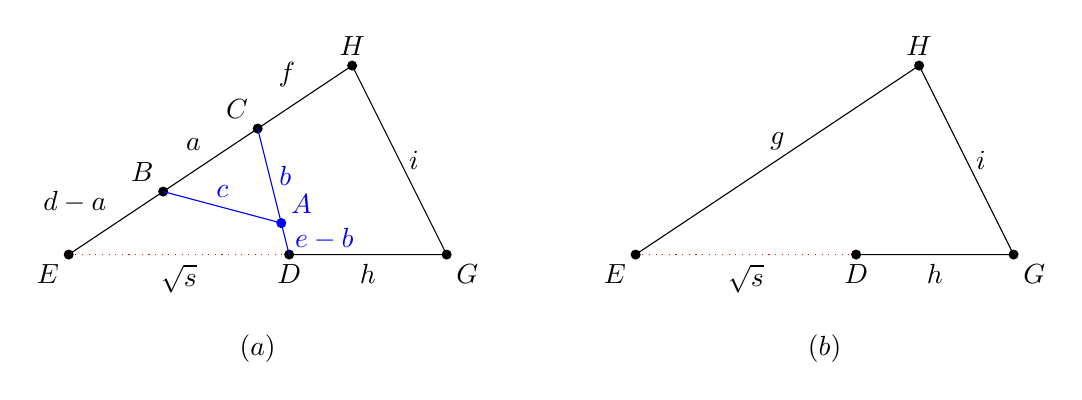
\begin{tikzpicture}
\begin{scope}[scale=0.4]
\begin{scope}
\draw[red,dotted] (0,0) -- node[below,black]{$\sqrt{s}$}++(7,0);
\draw[black,fill=black] (7,0) node[below]{$D$}  circle(4pt)
-- node[below]{$h$} ++(5,0) node[below right]{$G$} circle(4pt)
-- node[right]{$i$} ++(-3,6) node[above]{$H$} circle(4pt)
-- node[above left]{$f$} ++(-3,-2) node[above left]{$C$} circle(4pt)
-- node[above left]{$a$} ++(-3,-2) node[above left]{$B$} circle(4pt)
-- node[above left]{$d-a$} ++(-3,-2) node[below left]{$E$} circle(4pt);
\draw[blue,fill=blue] (7,0)
-- node[right]{$e-b$} ++(-.25,1) node[above right]{$A$} circle(4pt)
-- node[right]{$b$} ++(-.75,3)
   ++(+.75,-3)
-- node[above]{$c$} (3,2);
\draw[black](6,-3) node{$(a)$};
\end{scope}

\begin{scope}[shift={(18,0)}]
\draw[red,dotted] (0,0) -- node[below,black]{$\sqrt{s}$}++(7,0);
\draw[black,fill=black] (7,0) node[below]{$D$}  circle(4pt)
-- node[below]{$h$} ++(5,0) node[below right]{$G$} circle(4pt)
-- node[right]{$i$} ++(-3,6) node[above]{$H$} circle(4pt)
-- node[above]{$g$} ++(-9,-6) node[below left]{$E$} circle(4pt);
\draw[black](6,-3) node{$(b)$};
\end{scope}


\end{scope}
\end{tikzpicture}
\caption{The five strips intented to form an algebraic distance $\overline{EG} = \sqrt{s} + h$.}
\label{fig:alg-not-right}
\end{figure}

From figure \ref{fig:alg-not-right} $(a)$ we know $\sqrt{s}$ distance
between nodes $E$ and $D$ is produced by the three strips frame $a+d$, $b+e$ and $c$.
Using the law of cosines we calculate the angle $\theta = \angle{CED}$ in terms of $\sqrt{s}$:

\begin{align}
\cos\theta &= \frac{d^2 + (\sqrt{s})^2 - e^2}{2d\sqrt{s}} \nonumber\\
 &= \frac{(d^2 + s - e^2)\sqrt{s}}{2ds} \\
 &= \frac{m\sqrt{s}}{n} \label{eq:cos1}\\
 m &= d^2 + s - e^2 \\
 n &= 2ds
\end{align}

From figure \ref{fig:alg-not-right} $(a)$ we notice two sets of points are collinear:
$\{ E,B,C,H \}$ and $\{ E,D,G \}$. Using the law of cosines we calculate the 
angle $\theta = \angle{HEG}$ in terms of distances $g,\sqrt{s}+h,i$:

\begin{align}
\cos\theta &= \frac{g^2 + (\sqrt{s}+h)^2 - i^2}{2g(\sqrt{s}+h)} \nonumber\\
 &= \frac{g^2 + s + 2\sqrt{s}h + h^2 - i^2}{2g(\sqrt{s}+h)} \nonumber\\
 &= \frac{g^2 + s + h^2 - i^2+ 2\sqrt{s}h}{2g(\sqrt{s}+h)}
\end{align}

We multiply both numerator and denominator by $\sqrt{s}-h$ to eliminate the surd from denominator:
\begin{align}
\cos\theta &= \frac{(s + g^2 + h^2 - i^2)(\sqrt{s}-h) + 2\sqrt{s}h(\sqrt{s}-h)}
	{2g(\sqrt{s}+h)(\sqrt{s}-h)} \nonumber\\
 &= \frac{(s + g^2 + h^2 - i^2)(\sqrt{s}-h) + 2sh - 2\sqrt{s}h^2}
	{2g(s-h^2)} \nonumber\\ 
 &= \frac{-h(s + g^2 + h^2 - i^2 - 2s) + (s + g^2 + h^2 - i^2 - 2h^2)\sqrt{s}}
	{2g(s-h^2)} \nonumber\\ 
 &= \frac{h(s - g^2 - h^2 + i^2) + (s + g^2 - h^2 - i^2)\sqrt{s}}
	{2g(s-h^2)} \nonumber\\ 
 &= \frac{o + p\sqrt{s}}{q} \label{eq:cos2}\\
o &= h(s - g^2 - h^2 + i^2) \\
p &= s + g^2 - h^2 - i^2 \\
q &= 2g(s-h^2)
\end{align}

We compare both cosines equations \ref{eq:cos1} and \ref{eq:cos2}:
\begin{align}
\frac{m\sqrt{s}}{n} &= \frac{o + p\sqrt{s}}{q}
\end{align}
Since all variables are integers we need two conditions. First $o$ should be zero.
And second $\frac{m}{n} = \frac{p}{q}$.

For condition 1, we force $o$ to be zero:
\begin{align}
o &= 0 \nonumber\\
h(s - g^2 - h^2 + i^2) & = 0 \nonumber\\
s &= g^2 + h^2 - i^2 \label{eq:condition1}
\end{align}

For condition2, we force $m,n,p,q$ as:
\begin{align}
\frac{m}{n} &= \frac{p}{q} \nonumber\\
\frac{d^2 + s - e^2}{2ds} &= \frac{s + g^2 - h^2 - i^2}{2g(s-h^2)} \nonumber\\
\end{align}

We replace the value of $s$ of last equation RHS with the value of equation \ref{eq:condition1}
of condition 1:
\begin{align}
\frac{d^2 - e^2 + s}{ds} &= \frac{s + g^2 - h^2 - i^2}{g(s-h^2)} \nonumber\\
 &= \frac{g^2 + h^2 - i^2 + g^2 - h^2 - i^2}{g(g^2 + h^2 - i^2-h^2)} \nonumber\\
 &= \frac{2(g^2 - i^2)}{g(g^2 - i^2)} \nonumber\\
 &= \frac{2}{g} \nonumber\\
(d^2 - e^2 + s)g &= 2ds \label{eq:condition2}
\end{align}

\boxed{TODO: Examples!!!}



\section{Triangle pair frame}

\begin{figure}[H]
\centering
\begin{center}
\meccanoframetrianglepair{2}{3}{4} {3}{5}{7} {3pt}{1.0}{7}
\end{center}
\caption{Triangle pair frame.
We join triangles $\triangle{ABC}$ and $\triangle{DEF}$ in such a way vertices $C$ and $F$ coincide
and vertices $A,C,D,E$ be collinear. The result is a five strips frame. We are interested in the
distance $\overline{BE}$.}
\label{fig:tripair}
\end{figure}

Figure \ref{fig:tripair} shows a triangle pair frame. The triangles share a strip which contains four of the vertices.
The remaining two vertices are separated by distances of the form $\dfrac{\sqrt{F+G\sqrt{H}}}A$. With only five strips this frame is small and useful to make up the diagonals inside polygons we want to be rigid.

\subsection{Triangle pair algebra}

First we calculate the cosines:
\begin{align}
\cos\alpha &= \frac{a^2 + b^2 - c^2}{2ab}\nonumber\\
\cos\beta  &= \frac{d^2 + e^2 - f^2}{2de}\nonumber
\end{align}
We define integers $m,n,o,p$ to simplify cosines and get sines:
\begin{align}
(m, n) &\equiv (a^2 + b^2 - c^2, 2ab) \quad | m | \le n\\
(o, p) &\equiv (d^2 + e^2 - f^2, 2de) \quad | o | \le p\\
\cos\alpha &= \frac{m}n\\
\cos\beta  &= \frac{o}p\\
\sin\alpha &= \sqrt{1-\cos^2\alpha} = \frac{\sqrt{n^2 - m^2}}n\\
\sin\beta  &= \sqrt{1-\cos^2\beta} = \frac{\sqrt{p^2 - o^2}}p
\end{align}
Then, we use the cosines sum identity:
\begin{align}
\cos(\alpha+\beta) &= \cos\alpha\cos\beta - \sin\alpha\sin\beta \nonumber\\
 &= \left(\frac{m}n\right)\left(\frac{o}p\right)
  - \left(\frac{\sqrt{n^2 - m^2}}n\right)\left(\frac{\sqrt{p^2 - o^2}}p\right) \nonumber\\
 &= \frac{mo - \sqrt{(n^2 - m^2)(p^2 - o^2)}}{np}
\end{align}
Finally we can calculate the distance $g \equiv \overline{BE}$ using the law of cosines:
\begin{align}
g &\equiv \overline{BE}\nonumber\\
 &= \sqrt{a^2 + d^2 - 2ad\cos(\alpha+\beta)}\nonumber\\
 &= \sqrt{a^2 + d^2 - 2ad\left(\frac{mo - \sqrt{(n^2 - m^2)(p^2 - o^2)}}{np}\right)}\nonumber\\
 &= \sqrt{a^2 + d^2 - 2ad\left(\frac{mo - \sqrt{(n^2 - m^2)(p^2 - o^2)}}{4abde}\right)}\nonumber\\
 &= \sqrt{a^2 + d^2 - \frac{mo - \sqrt{(n^2 - m^2)(p^2 - o^2)}}{2be}}\nonumber\\
 &= \frac{\sqrt{4b^2e^2(a^2 + d^2) - 2bemo + 2be\sqrt{(n^2 - m^2)(p^2 - o^2)}}}{2be}
\end{align}
For the software we can define integers $A,F,G,H$ to calculate and reduce $g$:
\begin{align}
A &\equiv 2be\\
F &\equiv A^2(a^2+d^2) - Amo\\
G &\equiv A\\
H &\equiv (n^2-m^2)(p^2-o^2)\\
g &= \frac{\sqrt{F+G\sqrt{H}}}A
\end{align}

\subsection{Triangle pairs software}

We run a program to inspect triangle pairs having a given distance $g$. The software iterates
over the two triangles sides $(a,b,c)$ and $(d,e,f)$ up to a maximum strip length.
\\\\
Next example request distances of the form $\sqrt{46+18\sqrt{5}}$ up to strip length $10$:

%%----------- start
\begin{align*}
Folder &: \texttt{github.com/heptagons/meccano/frames}\\
Call &: \texttt{NewFrames().TrianglePairsTex(10, [46 18 5])}\end{align*}
\begin{align*}
(a,b,c) \oplus (d,e,f) &\mapsto g\\
\hline
%a=1...\\ 
%a=2...\\ 
(2,1,2) \oplus (3,3,3) &\mapsto \frac{\sqrt{46+18\sqrt{5}}}{2} \\
(2,1,2) \oplus (3,8,7) &\mapsto \frac{\sqrt{46+18\sqrt{5}}}{2} \\
(2,2,2) \oplus (3,6,6) &\mapsto \frac{\sqrt{46+18\sqrt{5}}}{2} \\
(2,3,4) \oplus (3,5,7) &\mapsto \frac{\sqrt{46+18\sqrt{5}}}{2} \\
(2,4,4) \oplus (3,8,7) &\mapsto \frac{\sqrt{46+18\sqrt{5}}}{2} \\
%a=3...\\ 
(3,3,3) \oplus (2,4,4) &\mapsto \frac{\sqrt{46+18\sqrt{5}}}{2} \\
%a=4...\\ 
(4,2,4) \oplus (6,6,6) &\mapsto \sqrt{46+18\sqrt{5}} \\
(4,4,4) \oplus (6,7,8) &\mapsto \sqrt{46+18\sqrt{5}} \\
%a=5...\\ 
%a=6...\\ 
(6,3,6) \oplus (4,4,4) &\mapsto \sqrt{46+18\sqrt{5}} \\
(6,3,6) \oplus (9,9,9) &\mapsto \frac{3\sqrt{46+18\sqrt{5}}}{2} \\
(6,6,6) \oplus (4,8,8) &\mapsto \sqrt{46+18\sqrt{5}} \\
(6,7,8) \oplus (9,9,9) &\mapsto \frac{3\sqrt{46+18\sqrt{5}}}{2} \\
%a=7...\\ 
%a=8...\\ 
%a=9...\\ 
%a=10...\\ 
\end{align*}
%%----------- end


\begin{figure}[H]
\centering
\begin{center}
\meccanoframetrianglepair{2}{1}{2} {3}{3}{3} {3pt}{1.0}{1} % last 1 is to show vertices A,B,C,D,E,F
\end{center}
\caption{Triangle pair frame $(2,1,2) \oplus (3,3,3)$ makes $\overline{BE} = \dfrac{\sqrt{46+18\sqrt{5}}}{2}$.}
\label{fig:tripair212333}
\end{figure}







\section{Two triangles with offsets}

\begin{figure}[H]
\centering
\begin{center}
% a,b,c,d,e,p,scale, x+g, g,h,i,j,k, x,p
\meccanoframefive{6}{5}{5}{3}{2}{3pt}{0.6} {7} {3}{4}{4}{3}{2} {3} (a)
\meccanoframefive{6}{5}{5}{0}{2}{3pt}{0.7} {7} {3}{4}{4}{0}{2} {3} (b)
\end{center}
\caption{Frame of two triangles with offsets. We construct two triangles $\triangle{ABC}$ and
$\triangle{GHI}$. Extending the strips we get four vertices $E,D,J,K$ which
can form four rigid distances of surd type: $\overline{DJ}, \overline{DK},
\overline{EJ}, \overline{EK}$.}
\label{fig:5strips}
\end{figure}

Figure \ref{fig:5strips} shows a frame with five strips. The frame has eleven variables:
\begin{align}
a &= \overline{BC}, \quad b = \overline{AC}, \quad c = \overline{AB}\\
d &= \overline{AE}, \quad e = \overline{AD}\\
f &= \overline{AG}\\
g &= \overline{HI}, \quad h = \overline{GI}, \quad i = \overline{GH}\\
j &= \overline{HJ}, \quad k = \overline{HK}
\end{align}

Assume vertex A is at the origin.
Let $\alpha = \angle{BAC}$, and $D_x,D_y$ the abscissa and orditate of vertex $D$ so we have:
\begin{align}
t &\equiv b^2 + c^2 - a^2\\
x &\equiv 4b^2c^2 - t^2\\
\cos\alpha &= \frac{t}{2bc}\\
\sin\alpha &= \frac{\sqrt{x}}{2bc}\\
D_x &= d\sin\alpha = \frac{d\sqrt{x}}{2bc}\\
D_y &= d\cos\alpha = \frac{dt}{2bc}\\
D_x^2 + D_y^2 &= d^2
\end{align}
Let $\delta = \angle{HGI}$ and $K_x,K_y$ the abscissa and ordinate of
vertex $K$ so we have:
\begin{align}
v &\equiv h^2 + i^2 - g^2\\
y &\equiv 4h^2i^2 - v^2\\
\cos\delta &= \frac{v}{2hi}\\
\sin\delta &= \frac{\sqrt{y}}{2hi}\\
K_x &= f + k\sin\delta = f + \frac{k\sqrt{y}}{2hi}\\
K_y &= -k\cos\delta = -\frac{kv}{2hi}\\
K_x^2 + K_y^2 &= f^2 + 2fk\sin\delta + k^2\\
 &= f^2+k^2 + \frac{fk\sqrt{y}}{hi}
\end{align}
We calculate the distance $\overline{DK}$:
\begin{align}
\overline{DK}^2 &= (D_x+K_x)^2 + (D_y+K_y)^2 \nonumber\\
 &= D_x^2 + 2D_xK_x + K_x^2 + D_y^2 + 2D_yK_y + K_y^2 \nonumber\\
 &= (D_x^2+D_y^2) + (K_x^2+K_y^2) + 2D_xK_x + 2D_yK_y \nonumber\\
 &= d^2 + f^2 + k^2 + \frac{fk\sqrt{y}}{hi}
  + 2\left(\frac{d\sqrt{x}}{2bc}\right)\left(f + \frac{k\sqrt{y}}{2hi}\right)
  + 2\left(\frac{dt}{2bc}\right)\left(-\frac{kv}{2hi}\right) \nonumber\\
 &= d^2 + f^2 + k^2 - \frac{dtkv}{2bchi} + \frac{fk\sqrt{y}}{hi}
  + \frac{df\sqrt{x}}{bc} + \frac{dk\sqrt{xy}}{2bchi}
\end{align}

\end{document}